\documentclass{article}
% translate with >> pdflatex -shell-escape <file>

% This file is used as unit test for pgfplots, copyright by Christian Feuersaenger.
% 
% See
%   http://pgfplots.sourceforge.net/pgfplots.pdf
% for pgfplots.
%
% Any required input files (for <plot table> or <plot file> or the table package) can be downloaded
% at
% http://www.ctan.org/tex-archive/graphics/pgf/contrib/pgfplots/doc/latex/
% and
% http://www.ctan.org/tex-archive/graphics/pgf/contrib/pgfplots/doc/latex/plotdata/

\usepackage{pgfplots}
\pgfplotsset{compat=newest}

\pagestyle{empty}

\input reverseaxis_shared.tex
\begin{document}

	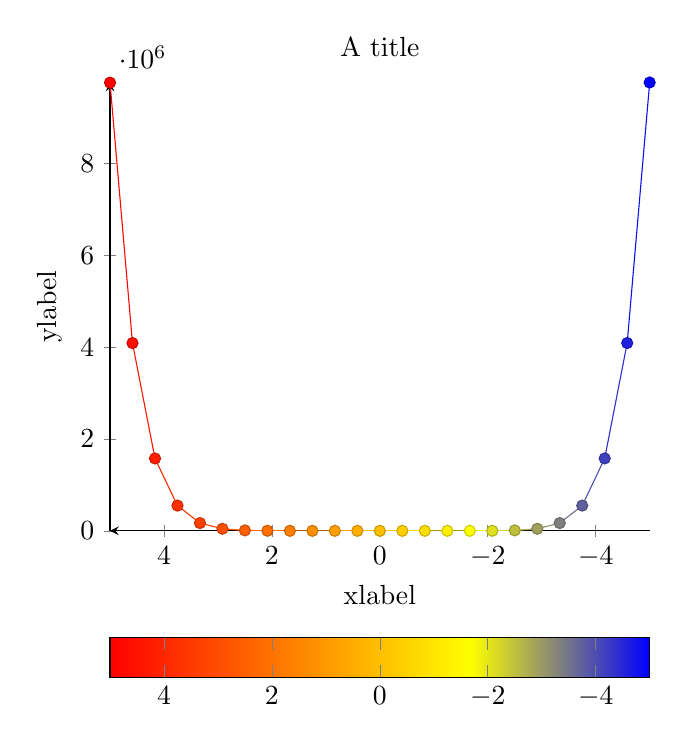
\begin{tikzpicture}
		\begin{axis}[
			axis lines=left,
			x dir=reverse,
			title=A title,
			xlabel=xlabel,
			ylabel=ylabel,
			colorbar horizontal,
			colorbar style={x dir=reverse},
		]
		\addplot+[mesh,scatter,scatter src=x] {x^10};
		\end{axis}
		\showanchorsafteraxis
	\end{tikzpicture}
\end{document}
